\chapter{Architektura rozwiązania}
\section{Architektura aplikacji}
Struktura aplikacji jest oparta na podziale wynikającym z wykorzystania frameworka Django. Zgodnie z tym założeniem projekt dzieli się na poszczególne moduły, które w rozumieniu platformy nazywane są paczkami.  W aplikacji można wyróżnić cztery podstawowe elementy kolejno odpowiadające za zarządzanie eksperymentami i użytkownikami, interfejs graficzny oraz aplikacja zbierająca wszystko w całość. Schemat modułów jest przedstawiony na Rys. \ref{rys4_packages}. 

\begin{figure}[htb]
	\centering
	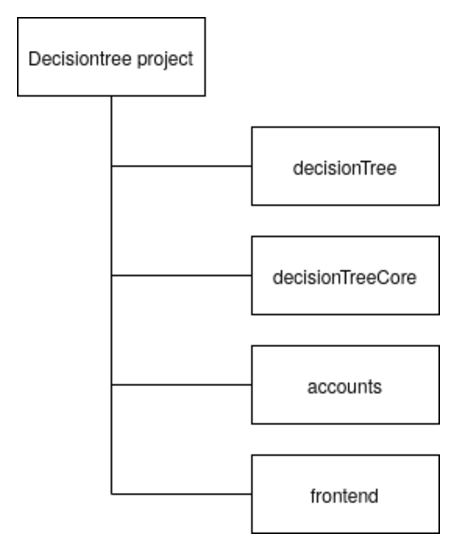
\includegraphics[height=8cm]{grafika/packages.eps}
	\caption{Podział projektu na moduły, źródło: opracowanie własne}
	\label{rys4_packages}
\end{figure}

\section{Przechowywanie danych}
w celu przechowywania wszelkich informacji została wykorzystana relacyjna baza danych PostgresSQL. Platforma ta jest postawiona na oddzielnym kontenerze w celu uzyskania większej stabilności i nie zależności od głównego modułu aplikacji. Schemat struktury wszystkich tabel został przedstawiony na Rys. \ref{rys5_database_schema}. Większość tabel wynika z samego zastosowania frameworka Django i DjangoRestFramework. Wykorzystując gotowe rozwiązana zostały zapewnione takie modele jak \enquote{auth\_user} odpowiadający za zapisywanie informacji o użytkownikach, czy też \enquote{authtoken\_token} mająca na celu przetrzymywanie tokenów autoryzacji. Do całej struktury zostały dodane dodatkowe tabele:
\begin{itemize}
	\item \enquote{decisionTreeCore\_experiment} przetrzymująca dane o eksperymentach,  
	\item \enquote{decisionTreeCore\_permissions} zawierająca informacje o prawach dostępowych do eksperymentu,
	\item \enquote{decisionTreeCore\_progress} składa się z pól określających postęp wykonywania doświadczenia.
\end{itemize}
\begin{figure}[htb]
	\centering
	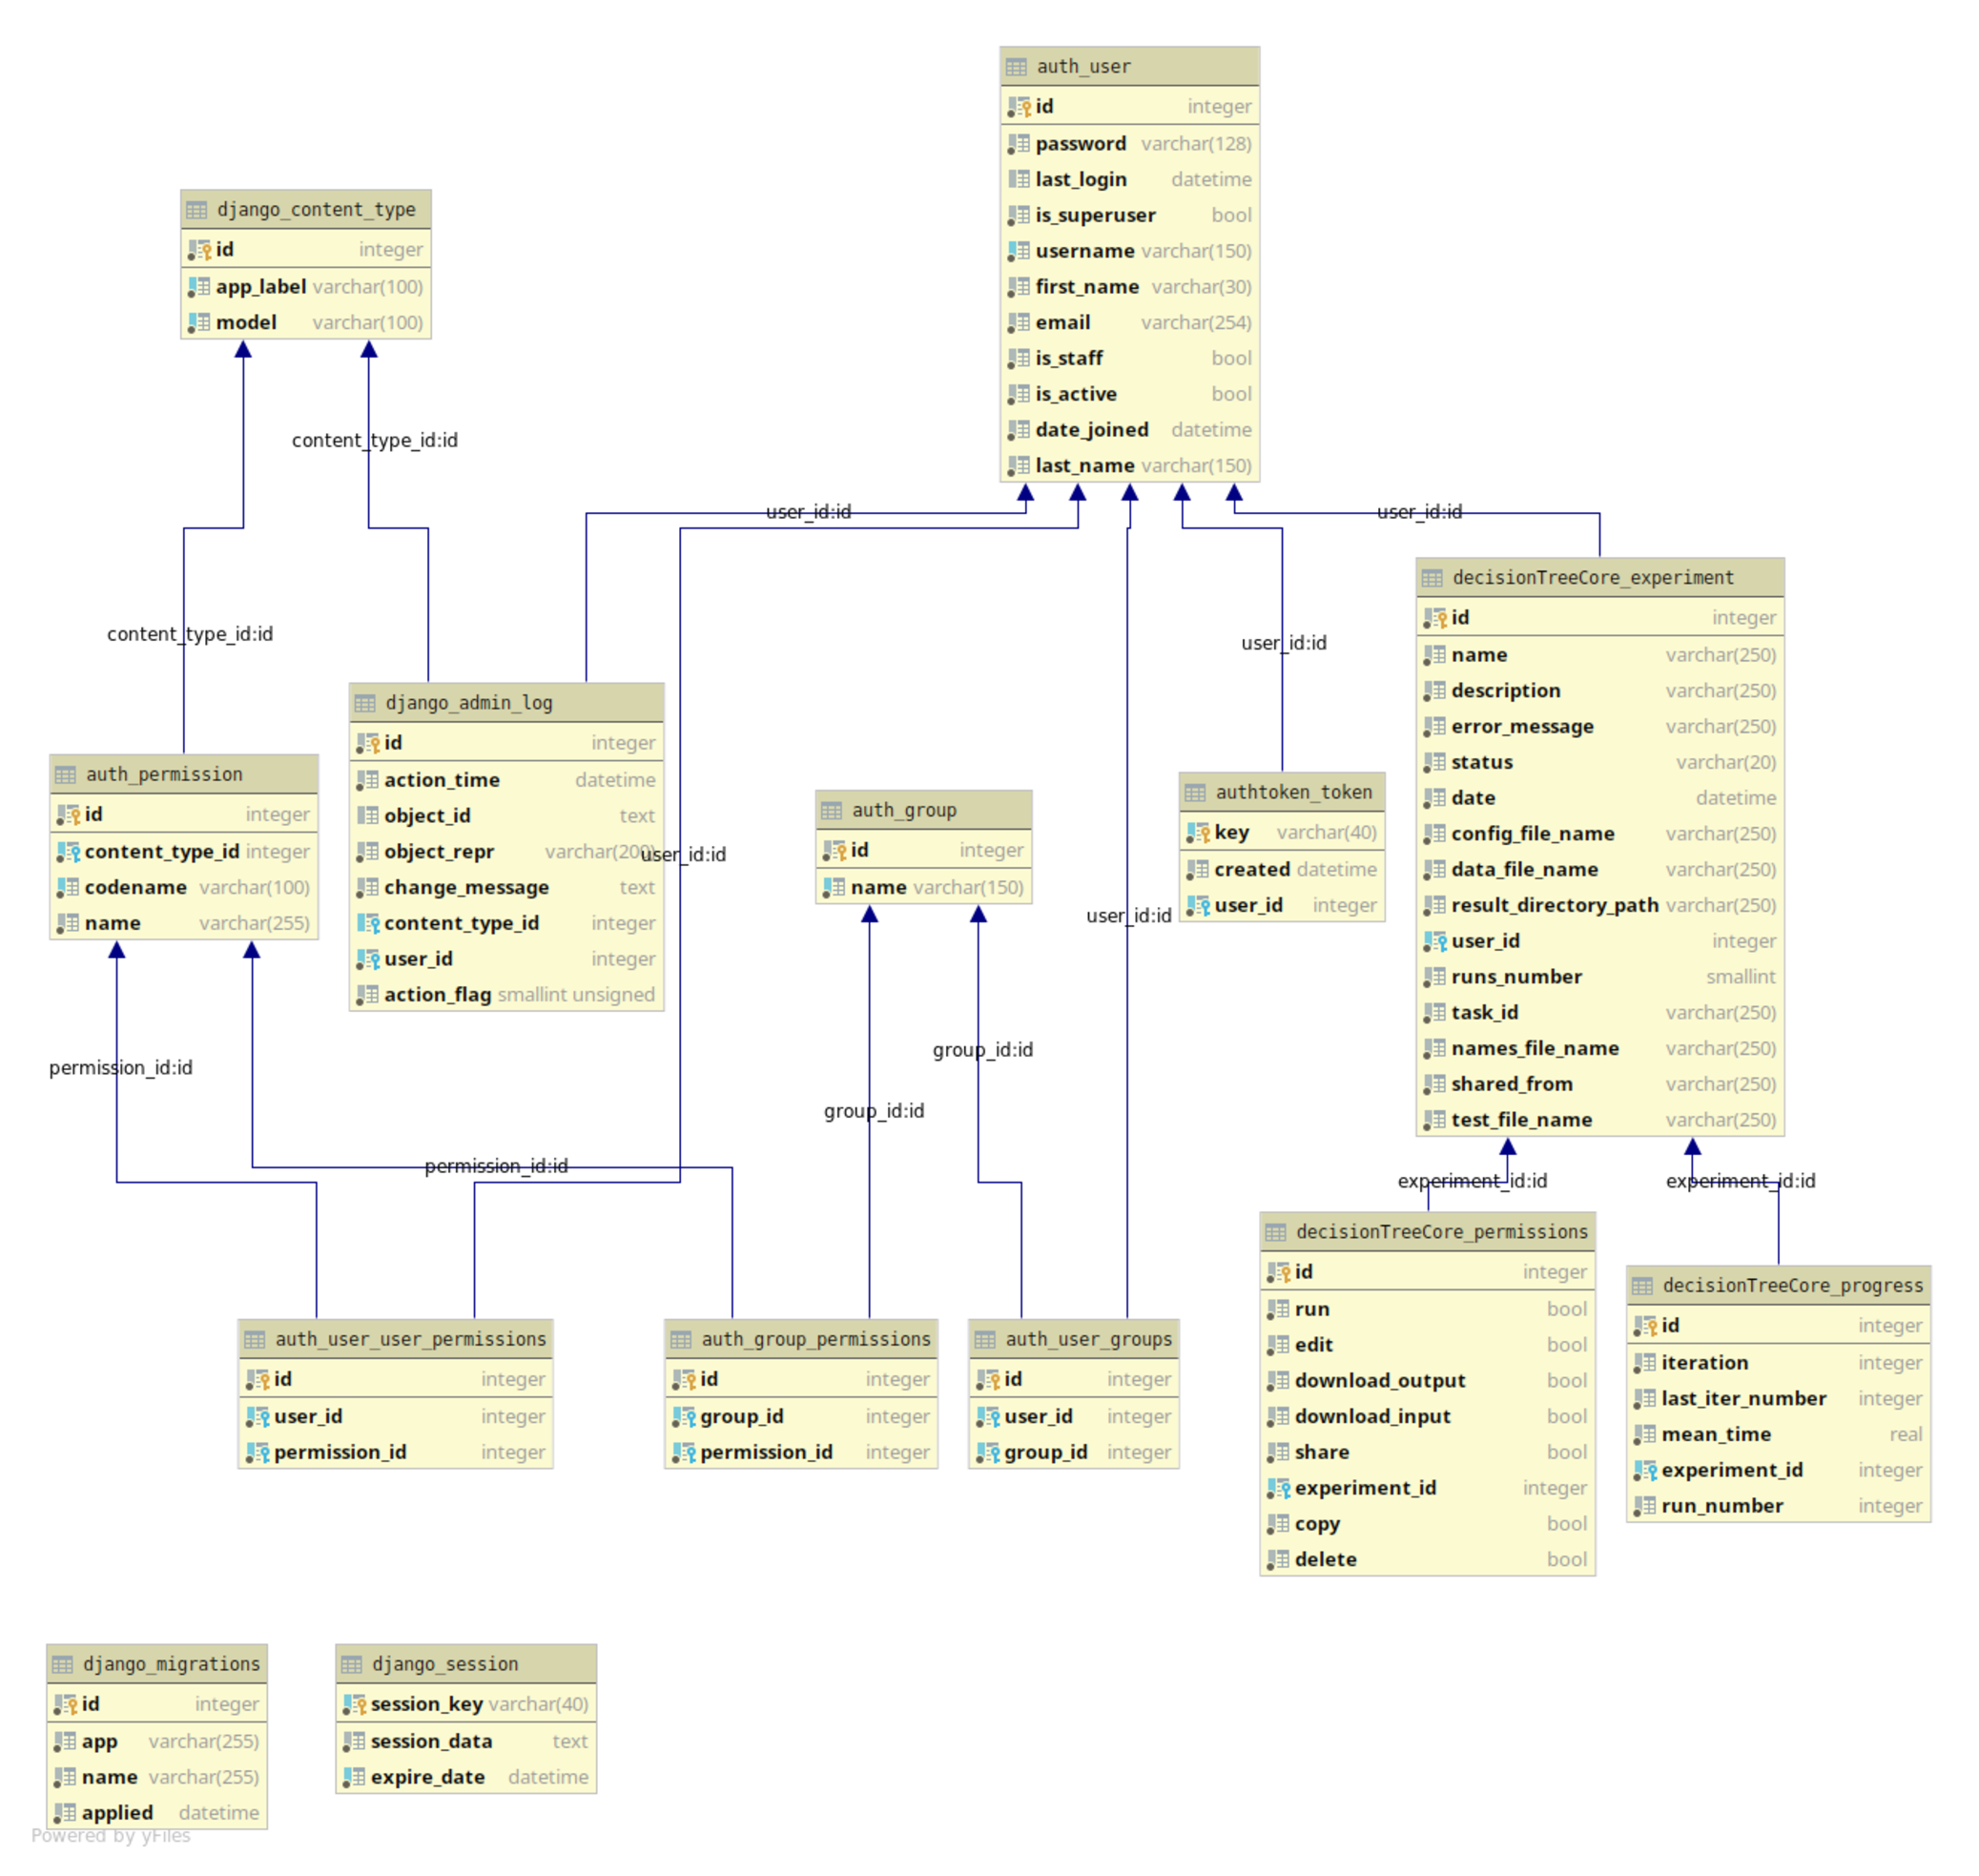
\includegraphics[angle=270, width=16cm]{grafika/database_schema.eps}
	\caption{Schemat bazy danych, źródło: opracowanie własne}
	\label{rys5_database_schema}
\end{figure}
Relacja pomiędzy nowo stworzonymi tabelami, a użytkownikiem została przedstawiona na Rys. \ref{rys6_database_schema}. 

\begin{table}[htb]
	\centering
	\begin{tabular}{|c|c|p{9cm}|}
		\hline
		\textbf{Nazwa pola} & \textbf{Typ} & \textbf{Opis} \\\hline
		id & integer & Klucz główny tabeli \\\hline
		name & varchar(50) & Nazwa eksperymentu\\\hline
		description & varchar(250) & Opis eksperymentu\\\hline
		error\_message & varchar(250) & Wiadomość o błędzie, który wystąpił podczas uruchomienia eksperyment\\\hline
		status & varchar(15) & Pole określające w jakim statusie znajduje się eksperyment. Możliwe wartości to: \enquote{Created}, \enquote{In queue}, \enquote{Running}, \enquote{Finished}, \enquote{Error}. Zmiana statusów następuje w trakcie przechodzenia eksperymentu przez kolejne etapy\\\hline
		data & datetime & Data stworzenia eksperymentu przez użytkownika\\\hline
		config\_file\_name & varchar(50) & Nazwa pliku konfiguracyjnego użytego w eksperymencie\\\hline
		data\_file\_name & varchar(50) & Nazwa pliku zawierającego zbiór uczący \\\hline
		test\_file\_name & varchar(50) & Nazwa pliku zawierającego zbiór testowy \\\hline
		names\_file\_name & varchar(50) & Nazwa pliku określającego nazwy klas oraz rodzaj zmiennych \\\hline
		result\_directory\_path & varchar(50) & Ścieżka do folderu z wynikami eksperymentu\\\hline
		user\_id & integer & ID użytkownika, który jest właścicielem eksperymentu \\\hline
		runs\_number & smalli & Pole określające ile przebiegów algorytmu ma się odbyć podczas uruchomienia eksperymentu w systemie GDT. Pełni ważną rolę przy tworzeniu paska postępu\\\hline
		task\_id & varchar(250) & Zawiera id zadania, które trafiło do robotnika Celery. Umożliwia zarządzanie danym zadaniem np. usunięcie z kolejki, lub anulowanie w trakcie trwania\\\hline
		shared\_from & varchar(250) & Pole pełni rolę zapisu informacji o poprzednich właścicielach. W wartością pola są nazwy użytkowników. Podczas kolejnych udostępnień do pola są dodawane po przecinku następne loginy  \\\hline
	\end{tabular}
	\caption[Opis pól encji \enquote{decisionTreeCore\_experiment}]{ Opis pól encji \enquote{decisionTreeCore\_experiment}}
	\label{tabela_1_schema_experiment}
\end{table}

 
\begin{figure}[htb]
	\centering
	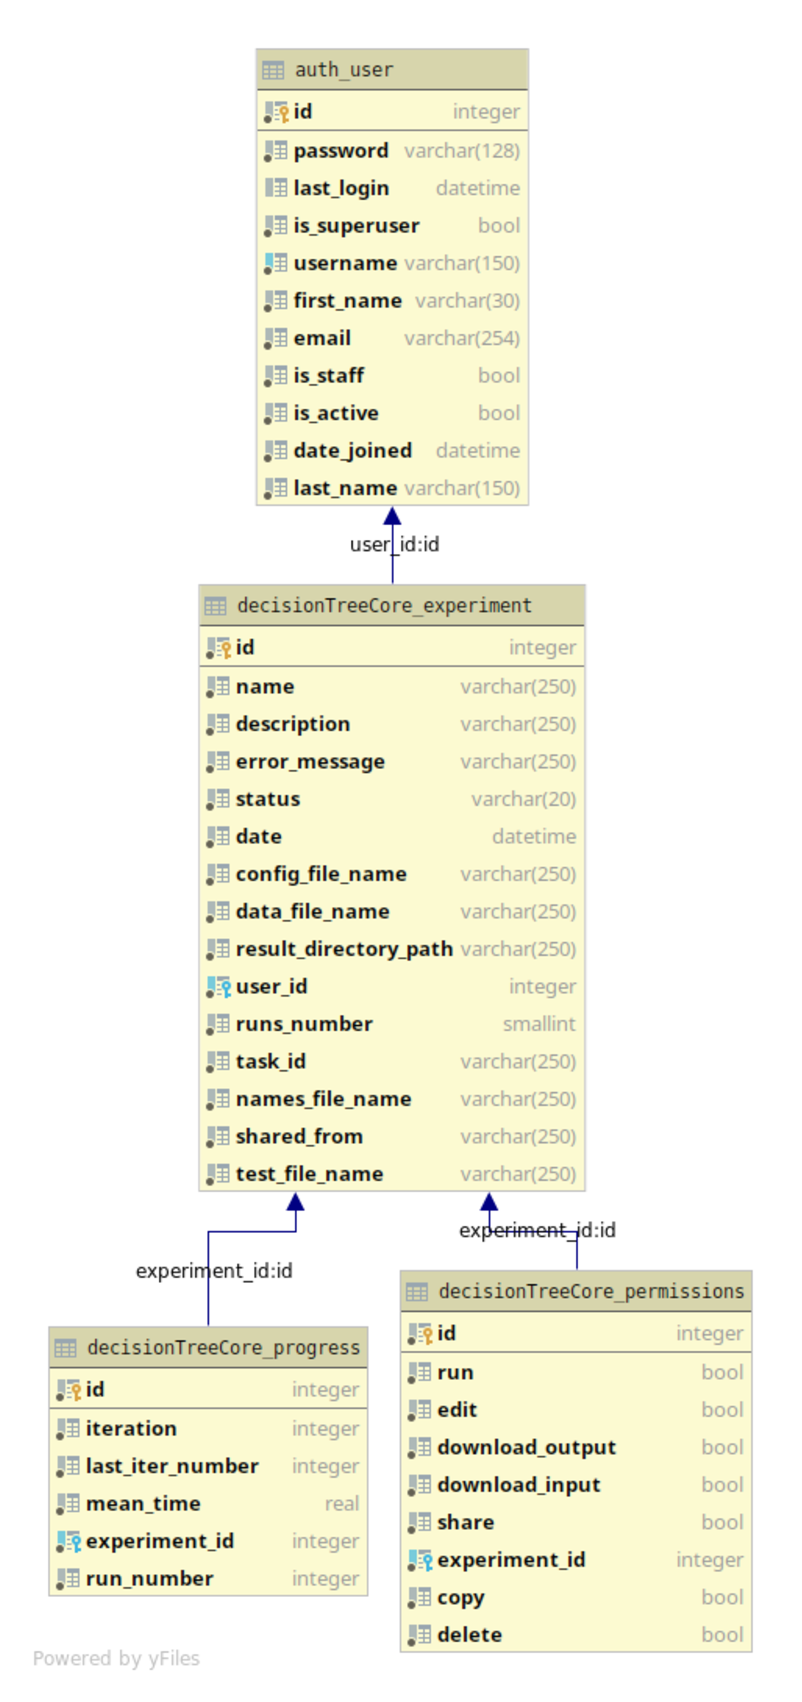
\includegraphics[height=14cm]{grafika/database_schema_2.eps}
	\caption{Schemat tabel dodatkowych, źródło: opracowanie własne}
	\label{rys6_database_schema}
\end{figure}

\section{Wdrożenie aplikacji}
